\documentclass[11pt]{article}


\usepackage[letterpaper,bindingoffset=0.2in,
            left=1in,right=1in,top=1in,bottom=1in,
            footskip=.25in]{geometry}
\usepackage{hyperref}
	\hypersetup{
			colorlinks=true,
			linkcolor=black,
			filecolor=magenta,      
			urlcolor=blue,
	}
\usepackage{graphicx}
	\graphicspath{ {images/} }
\usepackage{subcaption}
\usepackage{listings}
\usepackage{fancybox}


% Code to center a listing
% https://tex.stackexchange.com/questions/85489/how-to-center-a-lstlisting
\makeatletter
\newenvironment{CenteredBox}{% 
\begin{Sbox}}{% Save the content in a box
\end{Sbox}\centerline{\parbox{\wd\@Sbox}{\TheSbox}}}% And output it centered
\makeatother

	
\begin{document}


\title{COMP SCI 5401 FS2017 Assignment 2c}
\author{Stuart Miller\\\href{mailto:sm67c@mst.edu}{sm67c@mst.edu}}
\maketitle


\section{Overview}\label{sect:overview}

Assignment 2c provides an improvement to the Iterative Prisoner's Dilemma (IPD) problem by employing a coevolutionary Genetic Programming Search across single agents evaluated by a tit-for-tat strategy search. 


\section{Methodology}\label{sect:methodology}
As before, the algorithm works by generating a population of random trees (50\% full depth trees, 50\% grown tress), then iteratively generating children based on tree crossover from parents. Children are occasionally mutated, then simulated by playing tit-for-tat to obtain a fitness rating and added to the population. To obtain this fitness rating, each agents is plays a set number of rounds on a tit-for-tat strategy (the agent's opponent chooses what the agent itself did last). An option is also present to score each agent's fitness across multiple runs of IPD, with multiple randomized initial memories. Doing so allows for a more accurate fitness rating. After each generation, the population is thinned by removing poor agents chosen in a k-tournament. 

The main feature of this solution involves computing not only an absolute fitness for each agent, but also a composite coevolutionary fitness. This fitness is calculated after each generation is established (i.e. after all children have had their fitness independently evaluated). This composite fitness (referred to as "comp\_fitness" or variables prefixed with "comp" in code) is obtained by choosing a random sample of opponents from the population. Opponents are chosen without replacement. The absolute fitnesses of all chosen opponents and the agent itself are averaged and assigned to the agent in question as its composite fitness.

\section{Experimental Setup}\label{sect:exp_setup}

\begin{figure}[ht]
\begin{CenteredBox}
\lstinputlisting[lastline=21,frame=single,linewidth=4in,basicstyle=\small]{../../log/default.txt}
\end{CenteredBox}
\captionof{figure}{Configuration Values}
\label{fig:config}
\end{figure}

The following default configuration values were chosen (Figure \ref{fig:config}). Some algorithm parameters were dictated in the assignment (d, k, l, seedType, and evals). Termination is set to merely number of evals since this assignment dictated a 10,000 eval minimum. A mu and lambda of 100 and 50 were chosen. This allowed for rather sizable populations, but still a large number of generations before 10,000 evals. A low mutation rate was chosen as GP typically relies more heavily on recombination.  Survival selection was set to k-Tournaments with a k of 40. This allowed for sufficient exploration. As noted in Section \ref{sect:methodology}, there is an option to re-randomize an agents memory across multiple runs of IPD for more well-rounded fitness. This has been set to 5 here.  Finally, there is a small parsimony coefficient and plus survival strategy. These were simply inherited from the last assignment, since they worked well there.

The variation chosen for this assignment was the mutation operator. I thought it interesting that Koza states that small mutation sizes are preferred for GP, so an examination of this seems appropriate. The three values chosen were 5\%, 0\%, and 80\%. 5\% was the chosen default and seemed like an adequate approximation of Koza's recommended minimal value. 80\% was a sufficiently high number, and 0\% was chosen to see the effect of no mutation at all.

\section{Results}\label{sect:results}
\begin{figure}[ht]
\centering
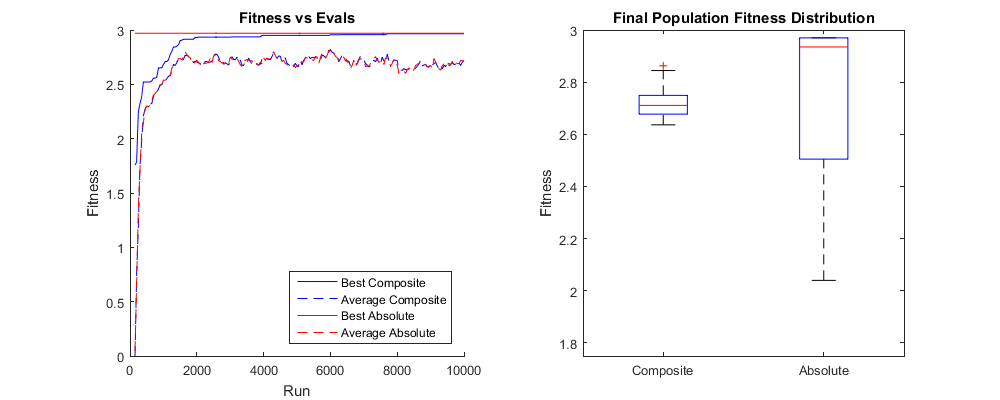
\includegraphics[width=6in]{default.png}
\captionof{figure}{Default Mutation (5\%) }
\label{fig:default}
\end{figure}
\begin{figure}[ht]
\centering
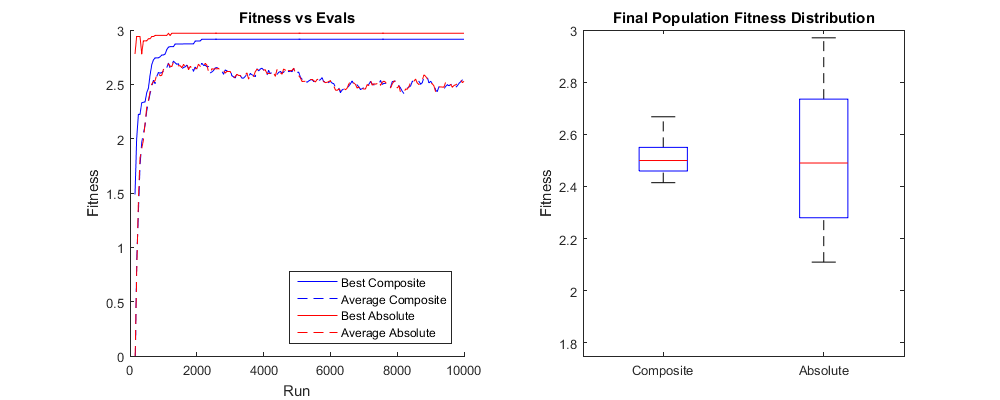
\includegraphics[width=6in]{high_mut.png}
\captionof{figure}{High Mutation (80\%) }
\label{fig:high_mut}
\end{figure}
\begin{figure}[ht]
\centering
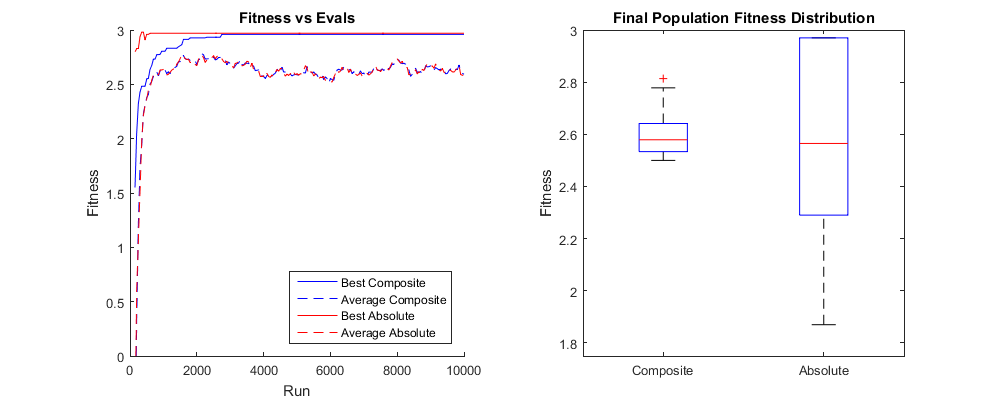
\includegraphics[width=6in]{no_mut.png}
\captionof{figure}{No Mutation (0\%)}
\label{fig:no_mut}
\end{figure}

\section{Discussion}\label{sect:discussion}
%The main problem with playing IPD tit-for-tat is that the agent very quickly learns that it can get into a pattern since the opponent is always guaranteed to do what it did last. It is very easy to an agent to get into a back-and-forth rhythm with its opponent with they simply alternate confessing and defecting. In such a way, all the agent has to do is choose what the opponent did an odd number of turns ago and it is guaranteed to score a 3 every time. Since there is a set number of startup round before payoffs are counted, the agent can establish this rhythm no matter what the initial memory is. This is evident in that the global best solution will almost always be O[1,3,5,...]. The agent is discouraged from branching out further because this would simply decrease its fitness do to the parsimony coefficient. The only way to break out of this would be to ditch the tit-for-tat strategy and implement a co-evolutionary approach. Perhaps even playing the against against a randomized opponent would fare better.

%This fallacy is visible in Figure \ref{fig:default}. Notice how the best run simply approaches 3 (minus the minimal parsimony deduction for have a very small tree). Also notice how useless the boxplot is due to the non-diverse final population. There are only three possible fitness values. The all scored the same but had different parsimony penalties for size 1, 2, or 3 trees.

\section{Conclusion}\label{sect:conclusion}




\end{document}